\documentclass{beamer}

\mode<presentation> {
	\usetheme{CambridgeUS}
	\usecolortheme{crane}
	\usefonttheme{default}
}

\usepackage{graphicx}
\usepackage{booktabs}
\usepackage{ragged2e}
\usepackage{minted}
\usepackage{lipsum}
\usepackage[export]{adjustbox}

%----------------------------------------------------------------------------------------
%	My Customized Settings
%----------------------------------------------------------------------------------------

\definecolor{UniBlue}{RGB}{83,121,170}
\definecolor{Black}{RGB}{125, 125, 125}
\definecolor{DarkBlue}{RGB}{50, 50, 153}
\definecolor{DarkGray}{RGB}{90,90,90}
\definecolor{LightGray}{RGB}{150,150,150}
\definecolor{TextGreen}{RGB}{115,155,15}
\definecolor{TextOrange}{RGB}{229, 148, 0}
\definecolor{Ocean}{RGB}{23,142,189}
\definecolor{BG}{RGB}{215,215,215}


\setbeamercolor{normal}{fg=DarkGray}
\setbeamercolor{title}{fg=UniBlue}
\setbeamercolor{frametitle}{fg=UniBlue}
\setbeamercolor{structure}{fg=UniBlue}
\setbeamercolor{normal text}{fg=DarkGray,bg=white}
\setbeamercolor{section number projected}{bg=UniBlue,fg=white}

\setbeamertemplate{itemize item}{\scriptsize\raise1.25pt\hbox{\donotcoloroutermaths$\blacktriangleright$}}
\setbeamertemplate{itemize subitem}{\tiny\raise1.5pt\hbox{\donotcoloroutermaths$\bullet$}}
\setbeamertemplate{itemize subsubitem}{\tiny\raise1.5pt\hbox{\donotcoloroutermaths$\blacksqaure$}}
\setbeamercolor{itemize item}{fg=darkred}
\setbeamercolor{itemize subitem}{fg=TextGreen}
\setbeamercolor{itemize subbody}{fg=LightGray}

\setbeamertemplate{enumerate subitem}{\insertenumlabel.\insertsubenumlabel}
\setbeamertemplate{enumerate subsubitem}{\insertenumlabel.\insertsubenumlabel.\insertsubsubenumlabel}
\setbeamertemplate{enumerate mini template}{\insertenumlabel}

\setbeamertemplate{navigation symbols}{}

\newcommand\VeryLargeFont{\fontsize{30}{15}\selectfont}
\newcommand\LargeFont{\fontsize{15}{15}\selectfont}
\newcommand\TinyFont{\fontsize{6}{6}\selectfont}

\setbeamertemplate{frametitle} {
  \nointerlineskip
  \begin{beamercolorbox}[sep=0.15cm,ht=1.3em,wd=\paperwidth]{frametitle}
    \vbox{}\vskip-2ex
    \strut\insertframetitle\strut
    \vskip-0.8ex
  \end{beamercolorbox}
}

\defbeamertemplate*{title page}{customized}[1][] {
	\centering
	\bigskip
	\bigskip
	\bigskip
	\usebeamercolor[fg]{title}\insertsubtitle\par
	\usebeamerfont{title}\inserttitle\par
	\usebeamerfont{subtitle}
	\bigskip
	\usebeamercolor[fg]{normal}
	\usebeamerfont{author}\insertauthor\par
	\usebeamerfont{institute}\insertinstitute\par
	\usebeamerfont{date}\insertdate\par
	\bigskip
	\bigskip
	\bigskip
	\bigskip
	\bigskip
	\usebeamercolor[fg]{titlegraphic}\inserttitlegraphic
}

%----------------------------------------------------------------------------------------
%	TITLE PAGE
%----------------------------------------------------------------------------------------
\title[Operating Systems of the IoT]{An Introduction to the Operating Systems of the IoT}
\author{Elahe Jalalpoor and Parham Alvani}
\institute[AUT] {
  Amirkabir University of Technology \\
  \medskip
  {\small\tt elahejalalpoor@gmail.com}\\
  {\small\tt parham.alvani@gmail.com}
  \medskip
}
\date{Jun 29, 2015}
\titlegraphic{\hspace*{5cm}
\includegraphics[width=2cm]{figs/aut_logo.jpeg}}

\begin{document}

\begin{frame}
\titlepage
\end{frame}

%----------------------------------------------------------------------------------------
%	PRESENTATION SLIDES
%----------------------------------------------------------------------------------------

%------------------------------------------------
\begin{frame}
	\frametitle{Outline}
	\begin{columns}[c]
		\begin{column}{30cm}
			\vspace{.1cm}
			\begin{itemize}
				\justifying
				\item Introduction
				\item IoT Requirements \& Challenges
				\item IoT OS
				\item Existing OSs
				\item Protocol stack
				\item Test \& Development Environments
				\item Conclusion
			\end{itemize}
		\end{column}
	\end{columns}
\end{frame}

%------------------------------------------------
\begin{frame}
	\frametitle{Introduction}
	\begin{columns}[c]
		\begin{column}{30cm}
			\vspace{.1cm}
			\begin{itemize}
				\justifying
				\item Introduction
				\begin{itemize}
					\item What is the IoT
				\end{itemize}
			\end{itemize}
		\end{column}
	\end{columns}
\end{frame}

%------------------------------------------------
\begin{frame}
	\begin{columns}
		\begin{column}{10cm}
			\vspace{2cm}
			\begin{block}{\centering\textcolor{darkred}{What is IoT\ldots}}
				\justifying
				The Internet of Things (IoT) is a scenario in which objects,
				animals or people are provided with unique identifiers and
				the ability to transfer data over a network without requiring human-to-human
				or human-to-computer interaction.\\
			\end{block}
		\end{column}
	\end{columns}
	\vspace{.75cm}
	\hspace*{8.5cm}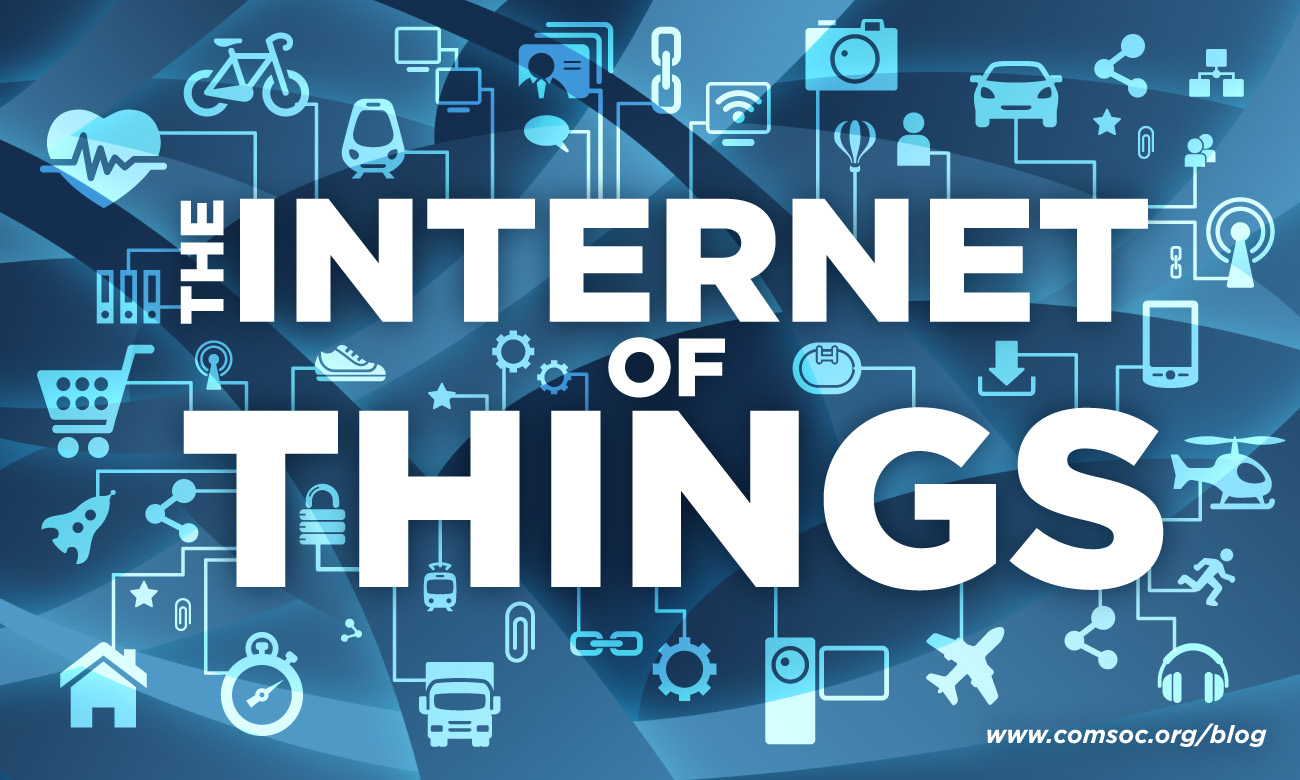
\includegraphics[width=3cm]{figs/Internet-of-Things-1.jpg}
\end{frame}

%------------------------------------------------
\begin{frame}
	\frametitle{IoT Requirements \& Challenges}
	\begin{columns}[c]
		\begin{column}{30cm}
			\vspace{.1cm}
			\begin{itemize}
				\justifying
				\item IoT Requirements \& Challenges
				\begin{itemize}
					\item Effect of the requirements on OS
				\end{itemize}
			\end{itemize}
		\end{column}
	\end{columns}
\end{frame}

%------------------------------------------------
\begin{frame}
	\frametitle{IoT Requirements \& Challenges}
	\begin{columns}[c]
		\begin{column}{30cm}
			\vspace{.1cm}
			\begin{itemize}
				\justifying
				\item Scalability
				\item Modularity
				\item Connectivity
				\item Reliability
			\end{itemize}
		\end{column}
	\end{columns}
	\vspace{.5cm}
	\hspace*{5.5cm} 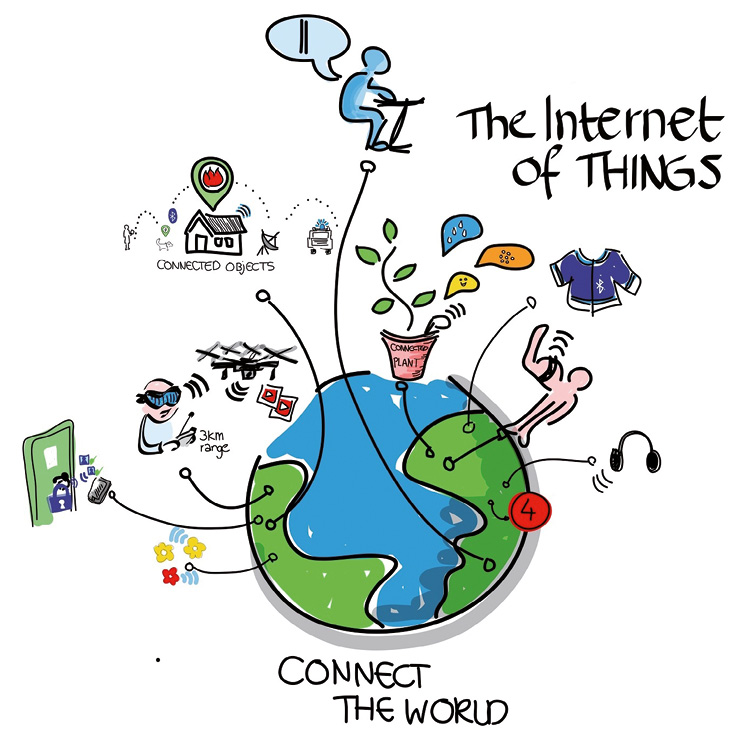
\includegraphics[width=5cm]{figs/Internet-of-Things-3.jpg}
\end{frame}

%------------------------------------------------
\begin{frame}
	\frametitle{Open Source Operating Systems for the IoT}
	\begin{columns}[c]
		\begin{column}{30cm}
			\vspace{.1cm}
			\begin{itemize}
				\justifying
				\item \textcolor{blue}{\href{http://www.freertos.org}{FreeRTOS}}
				\item \textcolor{blue}{\href{http://www.riot-os.org}{RIOT}}
				\item \textcolor{blue}{\href{http://www.contiki-os.org}{Contiki}}
				\item TinyOS
				\item Embedded Linux
				\item \textcolor{blue}{\href{http://www.openwsn.org}{OpenWSN}}
			\end{itemize}
		\end{column}
	\end{columns}
	\vspace{.5cm}
	\hspace*{5.5cm} 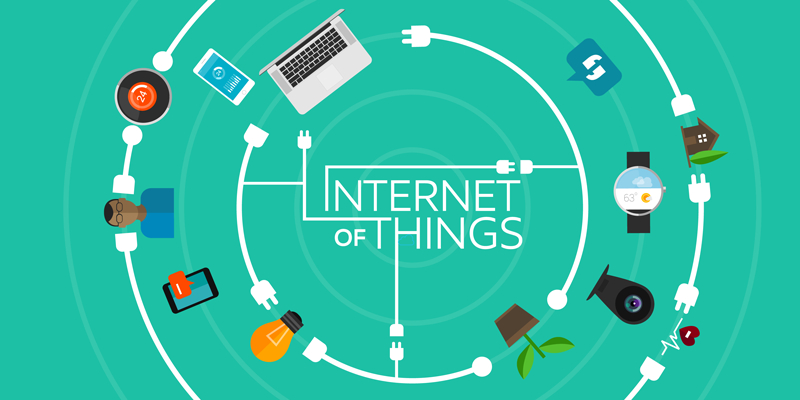
\includegraphics[width=5cm]{figs/Internet-of-Things-2.jpg}
\end{frame}

%------------------------------------------------
\begin{frame}
	\frametitle{FreeRTOS}
	\begin{columns}[c]
		\begin{column}{30cm}
			\vspace{.1cm}
			\begin{itemize}
				\justifying
				\item FreeRTOS is designed to be \textcolor{TextOrange}{small}
				and \textcolor{TextOrange}{simple}.
				\item The kernel itself consists of only three or four C files.
				\item It provides methods for multiple threads or tasks, mutexes,\\
				semaphores and software timers.
				\item Key features are \textcolor{TextGreen}{very small memory footprint},
				\textcolor{TextGreen}{low overhead},\\
				and \textcolor{TextGreen}{very fast execution}.
			\end{itemize}
		\end{column}
	\end{columns}
	\vspace{.5cm}
	\hspace*{5.5cm} 
\includegraphics[width=5cm]{figs/freertos-logo.jpg}	
\end{frame}

%------------------------------------------------
\begin{frame}
	\frametitle{RIOT}
	\begin{columns}[c]
		\begin{column}{30cm}
			\vspace{.1cm}
			\begin{itemize}
				\justifying
				\item RIOT is a \textcolor{TextOrange}{real-time}
				\textcolor{TextOrange}{multi-threading} operating system.
				\item RIOT is based on design objectives including:
				\begin{itemize}
					\justifying
					\item Energy-Efficiency
					\item Reliability
					\item Real-Time Capabilities
					\item Small Memory Footprint
					\item Modularity
					\item Uniform API Access\\
					independent of the underlying hardware\\
					(this API offers partial POSIX compliance)
				\end{itemize}
			\end{itemize}
		\end{column}
	\end{columns}
	\vspace{.5cm}
	\hspace*{5.5cm} 
\includegraphics[width=5cm]{figs/riot-logo.png}
\end{frame}

%------------------------------------------------
\begin{frame}
	\frametitle{Contiki}
	\begin{columns}[c]
		\begin{column}{30cm}
			\vspace{.1cm}
			\begin{itemize}
				\justifying
				\item Contiki is an open source operating system for \textcolor{TextOrange}{networked},\\
				\textcolor{TextOrange}{memory-constrained} systems
				\item Contiki provides three network mechanisms:
				\begin{itemize}
					\justifying
					\item The uIP stack, which provides IPv4 networking,
					\item The uIPv6 stack, which provides IPv6 networking,
					\item The Rime stack, which is a set of custom lightweight networking protocols\\
					designed specifically for low-power wireless networks.
				\end{itemize}
			\end{itemize}
		\end{column}
	\end{columns}
	\vspace{.5cm}
	\hspace*{5.5cm} 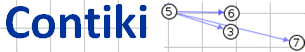
\includegraphics[width=5cm]{figs/contiki-logo.png}
\end{frame}

%------------------------------------------------
\begin{frame}
	\frametitle{TinyOS}
	\begin{columns}[c]
		\begin{column}{30cm}
			\vspace{.1cm}
			\begin{itemize}
				\justifying
				\item TinyOS is a \textcolor{TextOrange}{component-based} operating system and platform\\
				targeting wireless sensor networks.
				\item TinyOS is an embedded operating system written in the \textcolor{TextOrange}{nesC}\\
				\textcolor{TextOrange}{programming language} as a set of cooperating tasks and processes.
			\end{itemize}
		\end{column}
	\end{columns}
	\vspace{.5cm}
	\hspace*{5.5cm} 
\includegraphics[width=5cm]{figs/tinyos-logo.jpg}
\end{frame}

%------------------------------------------------
\begin{frame}
	\frametitle{Embedded Linux}
	\begin{columns}[c]
		\begin{column}{30cm}
			\vspace{.1cm}
			\begin{itemize}
				\justifying
				\item Embedded Linux is created using OpenEmbedded,\\
				the build framework for embedded Linux.
				\item OpenEmbedded offers a best-in-class cross-compile environment.
			\end{itemize}
		\end{column}
	\end{columns}
	\vspace{.5cm}
	\hspace*{5.5cm} 
\includegraphics[width=5cm]{figs/linux-logo.jpeg}
\end{frame}

%------------------------------------------------
\begin{frame}
	\frametitle{OpenWSN}
	\begin{columns}[c]
		\begin{column}{30cm}
			\vspace{.1cm}
			\begin{itemize}
				\justifying
				\item The goal of the OpenWSN project is to provide open-source\\
				implementations of a complete protocol stack based on Internet of\\
				Things standards, on a variety of software and hardware platforms.
			\end{itemize}
		\end{column}
	\end{columns}
	\vspace{.5cm}
	\hspace*{5.5cm} 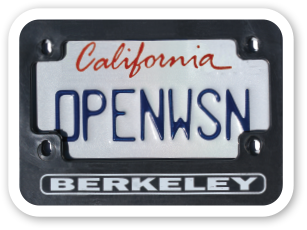
\includegraphics[width=5cm]{figs/openwsn-logo.png}
\end{frame}

%------------------------------------------------
\begin{frame}
	\frametitle{Comparison}
	\begin{columns}[c]
		\begin{column}{30cm}
			\hspace{0.9cm}
			\begin{tabular}{| c | c | c | c | c |}
				\hline
				OS & Min RAW & Min ROM & C Support & C++ Support \\ \hline
				Contiki & $< 2kB$ & $< 30kB$ & \textcolor{TextOrange}{Partial support} &
				\textcolor{red}{No support} \\ \hline
				Tiny OS & $< 1kB$ & $< 4kB$ & \textcolor{red}{No support} &
				\textcolor{red}{No support} \\ \hline
				Linux & $\sim 1MB$ & $\sim 1MB$ & \textcolor{TextGreen}{Full support} &
				\textcolor{TextGreen}{Full support} \\ \hline
				RIOT & $\sim 1.5kB$ & $\sim 5kB$ & \textcolor{TextGreen}{Full support} &
				\textcolor{TextGreen}{Full support} \\ \hline
			\end{tabular}
		\end{column}
	\end{columns}
	\vspace{.5cm}
	\hspace*{1cm}
	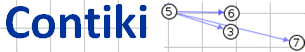
\includegraphics[width=2cm]{figs/contiki-logo.png}
	\hspace*{.5cm}
	
\includegraphics[width=2cm]{figs/tinyos-logo.jpg}
	\hspace*{.5cm}
	
\includegraphics[width=2cm]{figs/linux-logo.jpeg}
	\hspace*{.5cm}
	
\includegraphics[width=2cm]{figs/riot-logo.png}
\end{frame}

%------------------------------------------------
\begin{frame}
	\frametitle{Comparison}
	\begin{columns}[c]
		\begin{column}{30cm}
			\hspace{0.9cm}
			\begin{tabular}{| c | c | c | c |}
				\hline
				OS & Multi-Threading & Modularity & Real-Time \\ \hline
				Contiki & \textcolor{TextOrange}{Partial support} &
				\textcolor{TextOrange}{Partial support} &
				\textcolor{TextOrange}{Partial support} \\ \hline
				Tiny OS & \textcolor{TextOrange}{Partial support} &
				\textcolor{red}{No support} &
				\textcolor{red}{No support} \\ \hline
				Linux & \textcolor{TextGreen}{Full support} &
				\textcolor{TextOrange}{Partial support} &
				\textcolor{TextOrange}{Partial support} \\ \hline
				RIOT & \textcolor{TextGreen}{Full support} &
				\textcolor{TextGreen}{Full support} &
				\textcolor{TextGreen}{Full support} \\ \hline
			\end{tabular}
		\end{column}
	\end{columns}
	\vspace{.5cm}
	\hspace*{1cm}
	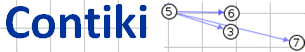
\includegraphics[width=2cm]{figs/contiki-logo.png}
	\hspace*{.5cm}
	
\includegraphics[width=2cm]{figs/tinyos-logo.jpg}
	\hspace*{.5cm}
	
\includegraphics[width=2cm]{figs/linux-logo.jpeg}
	\hspace*{.5cm}
	
\includegraphics[width=2cm]{figs/riot-logo.png}
\end{frame}

%------------------------------------------------
\begin{frame}
	\frametitle{Operating Systems Availability}
	\begin{columns}[c]
		\begin{column}{30cm}
			\hspace{0.9cm}
			\begin{tabular}{| c | c | c | c |}
				\hline
				OS & Wsn430 Node & M3 Node & A8 Node \\ \hline
				Contiki & \textcolor{TextGreen}{Full support} &
				\textcolor{TextGreen}{Full support} &
				\textcolor{red}{No support} \\ \hline
				Tiny OS & \textcolor{TextGreen}{Full support} &
				\textcolor{red}{No support} &
				\textcolor{red}{No support} \\ \hline
				Linux & \textcolor{red}{No support} &
				\textcolor{red}{No support} &
				\textcolor{TextGreen}{Full support} \\ \hline
				RIOT & \textcolor{TextGreen}{Full support} &
				\textcolor{TextGreen}{Full support} &
				\textcolor{red}{No support} \\ \hline
			\end{tabular}
		\end{column}
	\end{columns}
	\vspace{.5cm}
	\hspace*{1cm}
	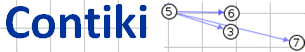
\includegraphics[width=2cm]{figs/contiki-logo.png}
	\hspace*{.5cm}
	
\includegraphics[width=2cm]{figs/tinyos-logo.jpg}
	\hspace*{.5cm}
	
\includegraphics[width=2cm]{figs/linux-logo.jpeg}
	\hspace*{.5cm}
	
\includegraphics[width=2cm]{figs/riot-logo.png}
\end{frame}

%------------------------------------------------
\begin{frame}
	\frametitle{Why Not Linux?}
	\begin{columns}[c]
		\begin{column}{12cm}
			\vspace{1cm}
			\begin{block}{\centering\textcolor{darkred}{Real-Time Linux}}
				\justifying
				Controlling a laser with Linux is crazy, but everyone in this room is crazy
				in his own way. So if you want to use Linux to control an industrial welding
				laser, I have no problem with your using PREEMPT\_RT.
				\vspace{.2cm}
				\hspace*{9.5cm}\footnotesize{- Linus Torvalds}
			\end{block}
		\end{column}
	\end{columns}
	\vspace{.5cm}
	\hspace*{.5cm}
	
\includegraphics[width=2cm]{figs/preempt-rt.png}
	\hspace*{3cm}
	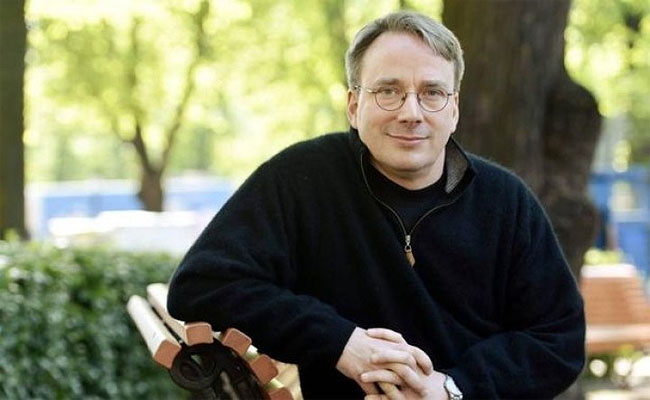
\includegraphics[width=5cm]{figs/linus-torvalds.jpg}
\end{frame}

%------------------------------------------------
\begin{frame}
	\frametitle{Why Not Linux?}
	\begin{columns}[c]
		\begin{column}{30cm}
			\vspace{.1cm}
			\begin{itemize}
				\justifying
				\item Linux certainly is a robust, developer-friendly OS
				\item Linux has a disadvantage when compared to a real-time operating system:
				\begin{itemize}
					\justifying
					\item Memory footprint
					\item It simply will not run on 8 or 16-bit MCUs
				\end{itemize}
				\item Linux will certainly have many uses in embedded devices, particularly\\
				ones that provide graphically rich user interfaces.
				\item There are thousands of applications for which Linux is ill suited.
			\end{itemize}
		\end{column}
	\end{columns}
	\vspace{.5cm}
	\hspace*{5.5cm} 
\includegraphics[width=5cm]{figs/tux-sad.png}
\end{frame}

%------------------------------------------------
\begin{frame}
	\frametitle{Close Source Operating Systems for the IoT}
	\begin{columns}[c]
		\begin{column}{30cm}
			\vspace{.1cm}
			\begin{itemize}
				\justifying
				\item \textcolor{blue}{\href{https://mbed.org/}{ARM mbed}}
				\item Huawei LiteOS
				\item Google Brillo
			\end{itemize}
		\end{column}
	\end{columns}
	\vspace{.5cm}
	\hspace*{5.5cm} 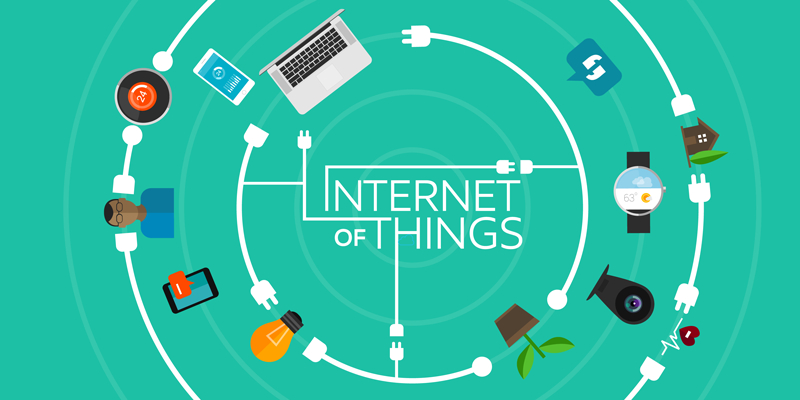
\includegraphics[width=5cm]{figs/Internet-of-Things-2.jpg}
\end{frame}

%------------------------------------------------
\begin{frame}
	\frametitle{ARM mbed}
	\begin{columns}[c]
		\begin{column}{30cm}
			\vspace{.1cm}
			\begin{itemize}
				\justifying
				\item Automation of power management
				\item Software asset protection and secure firmware updates for\\
				device security \& management
				\item Connectivity protocol stack support for Bluetooth® low energy,\\
				Cellular, Ethernet, Wi-fi, Zigbee IP, Zigbee NAN, 6LoWPAN
			\end{itemize}
		\end{column}
	\end{columns}
	\vspace{.5cm}
	\hspace*{5.5cm} 
\includegraphics[width=5cm]{figs/ARM-mbed-logo.png}
\end{frame}

%------------------------------------------------
\begin{frame}
	\frametitle{Huawei LiteOS}
	\begin{columns}[c]
		\begin{column}{30cm}
			\vspace{.1cm}
			\begin{itemize}
				\justifying
				\item The company says that its \textcolor{TextOrange}{LiteOS} is
				the \textcolor{TextGreen}{lightest} software of\\
				its kind and can be used to power a range of smart devices
			\end{itemize}
		\end{column}
	\end{columns}
	\vspace{.5cm}
	\hspace*{5.5cm} 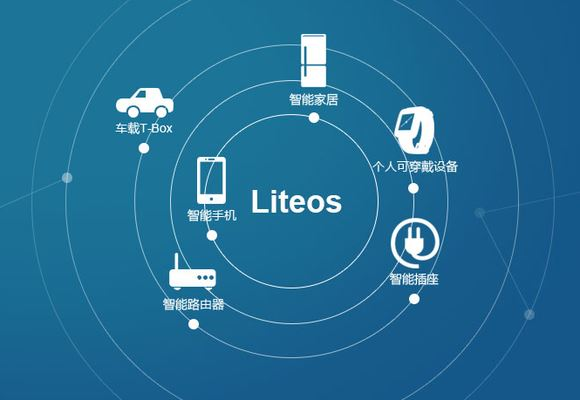
\includegraphics[width=5cm]{figs/huawei-liteos-logo.jpg}
\end{frame}

%------------------------------------------------
\begin{frame}
	\frametitle{Google Brillo}
	\begin{columns}[c]
		\begin{column}{30cm}
			\vspace{.1cm}
			\begin{itemize}
				\justifying
				\item Brillo is \textcolor{TextGreen}{derived} from Android
				but \textcolor{TextGreen}{polished} to just the lower levels.
				\item It supports Wi-Fi, Bluetooth Low Energy, and other Android things.
			\end{itemize}
		\end{column}
	\end{columns}
	\vspace{.5cm}
	\hspace*{5.5cm} 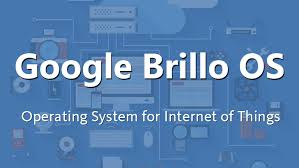
\includegraphics[width=5cm]{figs/google-brillo-logo.jpeg}
\end{frame}

%------------------------------------------------
\begin{frame}
	\frametitle{Internet Usage and Protocols for the IoT}
	\begin{columns}[c]
		\begin{column}{30cm}
			\vspace{.1cm}
			\begin{itemize}
				\justifying
				\item Can you build an IoT system with familiar Web technologies?
			\end{itemize}
		\end{column}
	\end{columns}
	\vspace{.5cm}
	\hspace*{5.5cm}
\end{frame}

%------------------------------------------------
\begin{frame}
	\frametitle{Internet Usage and Protocols for the IoT}
	\begin{columns}[c]
		\begin{column}{30cm}
			\vspace{.1cm}
			\begin{itemize}
				\justifying
				\item Can you build an IoT system with familiar Web technologies?
				\item Yes you can, although the result would not be as \textcolor{Ocean}{efficient} as\\
				with the \textcolor{TextGreen}{newer protocols}.
			\end{itemize}
		\end{column}
	\end{columns}
	\vspace{.5cm}
	\hspace*{5.5cm}
\end{frame}

%------------------------------------------------
\begin{frame}
	\frametitle{Internet Usage and Protocols for the IoT}
	\vspace{.5cm}
	\hspace*{1.5cm} 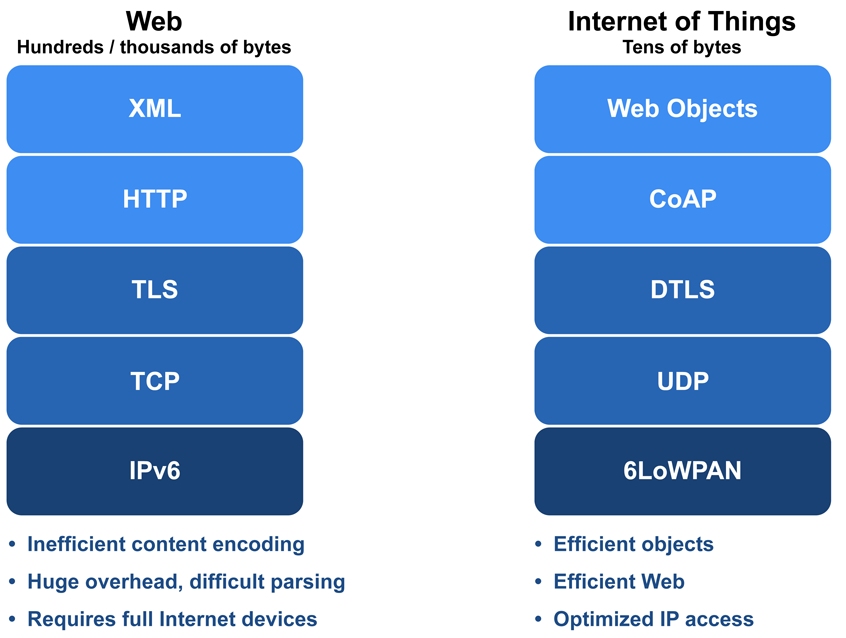
\includegraphics[width=10cm]{figs/Web-and-IoT-Stacks.png}
\end{frame}

%------------------------------------------------
\begin{frame}
	\frametitle{Internet Usage and Protocols for the IoT}
	\vspace{.25cm}
	\hspace*{.75cm} 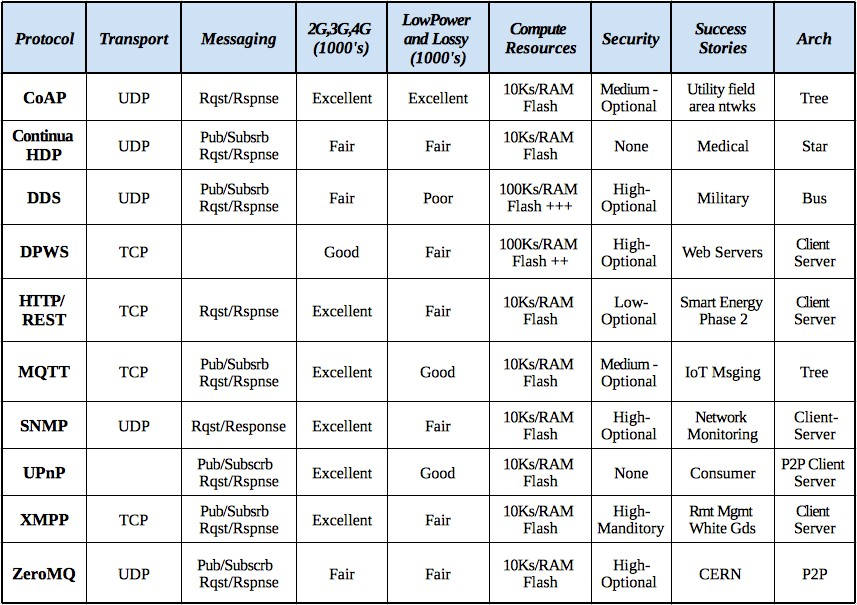
\includegraphics[width=10.5cm]{figs/iot-network-protocols.jpeg}
\end{frame}

%------------------------------------------------
\begin{frame}
	\frametitle{Modularity}
	\begin{columns}[c]
		\begin{column}{30cm}
			\vspace{.1cm}
			\begin{itemize}
				\justifying
				\item IoT device will require a modular operating system that separates\\
				\textcolor{TextGreen}{the core kernel} from
				\textcolor{TextOrange}{middleware},
				\textcolor{TextOrange}{protocols},
				and \textcolor{TextOrange}{applications}.
			\end{itemize}
		\end{column}
	\end{columns}
	\vspace{.5cm}
	\hspace*{5.5cm}
\end{frame}

%------------------------------------------------
\begin{frame}
	\frametitle{Multi-Tasking, Thread Model}
	\begin{columns}[c]
		\begin{column}{30cm}
			\vspace{.1cm}
			\begin{itemize}
				\justifying
				\item Most RTOS products on the market are thread model.
				\item \textcolor{TextGreen}{Tasks} are now called \textcolor{TextGreen}{threads}.
				\item All the \textcolor{TextOrange}{tasks} code and data occupy
				\textcolor{Ocean}{the same address space},\\
				along with that of the RTOS itself.
			\end{itemize}
		\end{column}
	\end{columns}
	\vspace{.5cm}
	\hspace*{5.5cm} 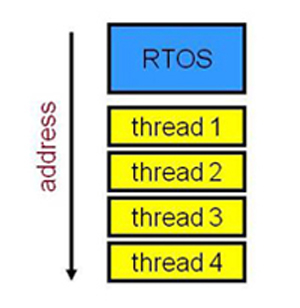
\includegraphics[width=5cm]{figs/thread-model.jpg}
\end{frame}

%------------------------------------------------
\begin{frame}
	\frametitle{Event-Driven, Non-Blocking I/O Model}
	\begin{columns}[c]
		\begin{column}{30cm}
			\vspace{.1cm}
			\begin{itemize}
				\justifying
				\item Networking Event-Driven
				\item Non-Blocking I/O
			\end{itemize}
		\end{column}
	\end{columns}
	\vspace{.5cm}
	\hspace*{5.5cm} 
\includegraphics[width=5cm]{figs/io.png}
\end{frame}

%------------------------------------------------
\begin{frame}
	\vspace{1cm}
	\begin{Huge}
		\begin{center}
			\usebeamercolor[fg]{title}Questions?
		\end{center}
	\end{Huge}
\end{frame}

\end{document}
